\documentclass[a4paper,12pt,oneside]{article}

\usepackage[T1]{fontenc}
\usepackage[utf8]{inputenc}
\usepackage[french]{babel}
\usepackage{csquotes}
\usepackage{lmodern}
\usepackage[a4paper,top=2.5cm,bottom=2.5cm,left=2.5cm,right=2.5cm]{geometry}
\usepackage{graphicx}
\usepackage{tikz}
\usetikzlibrary{angles,quotes,arrows.meta,decorations.pathreplacing,calc}
% Palette des schémas (reprise de la présentation intermédiaire)
\definecolor{heigred}{HTML}{D0002B}
\definecolor{deepblue}{HTML}{17324D}
\definecolor{softblue}{HTML}{E8F1F8}
\definecolor{softred}{HTML}{FBE9ED}
\definecolor{softgreen}{HTML}{E8F5EE}
\definecolor{mutedgray}{HTML}{6B7280}
\definecolor{linegray}{HTML}{D7DEE8}
\definecolor{camorange}{HTML}{C26A0F}
\definecolor{lasergreen}{HTML}{1F9D55}
\usepackage{booktabs}
\usepackage{array}
\usepackage{longtable}
\usepackage{float}
\usepackage{setspace}
\usepackage{hyperref}
\usepackage[backend=biber,style=numeric,sorting=none]{biblatex}
\usepackage{fancyhdr}
\usepackage{lastpage}
\usepackage{pdfpages}
\usepackage{subcaption}

% Metadonnees du rapport PMD
\newcommand{\projetNom}{Scanner 3D}
\newcommand{\versionDocument}{V1}
\newcommand{\filiere}{Projets Multidisciplinaires 2026}
\newcommand{\auteurs}{%
Marchand Luc, EAI\\
Stamm Tim, ROCM\\
Weber Jason, EAI\\
Fuentes Hadrien, EAI\\
Berthoud Tom, EAI%
}
\newcommand{\professeurRepondant}{Bornand Cédric}
\newcommand{\dateDocument}{\today}
\newcommand{\departement}{Departement TIC / TIN}
\newcommand{\uniteEnseignement}{Projet multidisciplinaire (PMD)}


\hypersetup{
  colorlinks = true,
  linkcolor  = black,
  urlcolor   = blue,
  citecolor  = black,
  pdftitle   = {\projetNom - Rapport technique}
}
\addbibresource{references.bib}

\setlength{\parindent}{0pt}
\setlength{\parskip}{0.4em}
\setlength{\headheight}{15pt}
\onehalfspacing

\fancypagestyle{rapport}{
  \fancyhf{}
  \fancyhead[L]{\projetNom}
  \fancyhead[R]{Rapport technique - \versionDocument}
  \fancyfoot[L]{\dateDocument}
  \fancyfoot[R]{\thepage/\pageref{LastPage}}
  \renewcommand{\headrulewidth}{0.4pt}
  \renewcommand{\footrulewidth}{0.4pt}
}

\begin{document}

\hypersetup{pageanchor=false}
\thispagestyle{empty}

\begin{center}
  
\includegraphics[height=2cm]{images/HEIG-VD_logo.png}
  \hfill
  
\includegraphics[height=2cm]{images/logo_hesso.pdf}
\end{center}

\vspace*{1.5cm}

\begin{center}
  {\Large \projetNom}\\[0.4cm]
  {\Large Rapport technique - \versionDocument}\\[0.3cm]
  {\large \filiere}
\end{center}

\vfill

\begin{center}
  \begin{tabular}{@{}lp{9.5cm}@{}}
    \textbf{Departement:} & \departement \\
    \textbf{Unite d'enseignement:} & \uniteEnseignement \\
    \textbf{Redige par:} & \begin{tabular}[t]{@{}l@{}}\auteurs\end{tabular} \\
    \textbf{Professeur repondant:} & \professeurRepondant \\
    \textbf{Date:} & \dateDocument
  \end{tabular}
\end{center}

\vspace*{1.2cm}

\clearpage

\pagestyle{rapport}
\pagenumbering{roman}
\setcounter{page}{2}
\hypersetup{pageanchor=true}

\section*{Historique du document}
\addcontentsline{toc}{section}{Historique du document}

\begin{longtable}{@{}p{2.8cm}p{3.2cm}p{8.2cm}@{}}
\toprule
\textbf{Version} & \textbf{Date} & \textbf{Changements} \\
\midrule
\endfirsthead
\toprule
\textbf{Version} & \textbf{Date} & \textbf{Changements} \\
\midrule
\endhead
V0.1 & 15.02.2026 & Création du squelette de rapport \\
V0.5 & 11.03.2026 & Alignement sur le cahier des charges V2 \\
V1 & 27.04.2026 & Version intermédiaire (prototype mono-caméra) \\
\versionDocument & \dateDocument & Version finale : passage double caméra, fusion et reconstruction, budget et résultats finaux \\
\bottomrule
\end{longtable}

\section*{References normatives}
\addcontentsline{toc}{section}{References normatives}

Les documents suivants cites dans le texte constituent, pour tout ou partie de leur contenu,
des exigences du present document.

\begin{longtable}{@{}p{4.2cm}p{10cm}@{}}
\toprule
\textbf{Norme} & \textbf{Description} \\
\midrule
\endfirsthead
\toprule
\textbf{Norme} & \textbf{Description} \\
\midrule
\endhead
CDC-Vxx & Cahier des charges fonctionnel - Vxx \\
ISO/IEC Directives Part 2:2016 & Principes et regles de structure et de redaction des documents ISO et IEC \\
OMG UML 2.5.1 & Unified Modeling Language pour l'ingenierie logicielle \\
\bottomrule
\end{longtable}

\section*{Abréviations}
\addcontentsline{toc}{section}{Abréviations}

Cette section précise les terminologies techniques et acronymes propres
au projet.

\begin{longtable}{@{}p{3cm}p{13cm}@{}}
\toprule
\textbf{Terme} & \textbf{Définition} \\
\midrule
\endfirsthead
\toprule
\textbf{Terme} & \textbf{Définition} \\
\midrule
\endhead
CDC      & Cahier des charges \\
CSI      & Camera Serial Interface (bus caméra du Raspberry Pi) \\
FS / FT / FC & Fonctions de Service / Techniques / de Contrainte \\
GPIO     & General Purpose Input/Output \\
HEIG-VD  & Haute École d'Ingénierie et de Gestion du Canton de Vaud \\
KDTree   & K-Dimensional Tree (structure d'indexation spatiale) \\
MakeLab  & Laboratoire de prototypage et de fabrication de la HEIG-VD \\
NEMA     & National Electrical Manufacturers Association (norme moteurs) \\
OBJ      & Format de fichier de modèle 3D (Wavefront) \\
PMD      & Projet multidisciplinaire \\
SSE      & Server-Sent Events \\
STL      & STereoLithography (format de maillage 3D) \\
USB      & Universal Serial Bus \\
MDF      & Medium Density Fiberboard (panneau de fibres de bois) \\
PLA      & Polylactic Acid (matériau d'impression 3D) \\
\bottomrule
\end{longtable}


\clearpage
\begingroup
\setstretch{1.1}
\tableofcontents
\endgroup
\clearpage
\begingroup
\setstretch{1.1}
\listoffigures
\endgroup
\clearpage
\begingroup
\setstretch{1.1}
\listoftables
\endgroup
\clearpage

\pagenumbering{arabic}
\setcounter{page}{1}

\section{Introduction}

\subsection{Contexte}
Ici, presenter le contexte du projet, son cadre et ses contraintes principales.

\subsection{Etat de l'art}
Resumer les solutions existantes et la valeur ajoutee de votre approche.

\subsection{But et objectifs}
Formuler la problematique puis lister les objectifs mesurables du projet (SMART).

\subsection{Planification}
Presenter la repartition du travail, les jalons et les livrables.

\section{Conception mécanique}

\subsection{Architecture mécanique}

Le scanner se présente sous la forme d'une boîte fermée de dimensions
extérieures inférieures à $500\times500\times500$\,mm pour une masse
totale inférieure à 15\,kg (exigence \textbf{E21}). L'architecture
est pensée pour une intégration directe dans l'environnement du
MakeLab de la HEIG-VD (FC3).

Le système s'organise autour de trois sous-ensembles :

\begin{itemize}
  \item \textbf{Plateau rotatif motorisé} (FT7, \textbf{E15}) :
        support de l'objet à numériser, entraîné par un moteur
        pas-à-pas NEMA\,17 couplé à un étage de transmission
        (courroie ou réduction directe, à figer).
  \item \textbf{Bâti de mesure} : supporte la caméra Pi\,Camera\,3
        et le module laser ligne vert dans une géométrie fixe et
        calibrée (angle connu, exigence \textbf{E12}).
  \item \textbf{Carter} : couvercle amovible équipé d'un
        micro-interrupteur de sécurité (SW1) assurant la coupure
        automatique du laser à l'ouverture (\textbf{E19}).
\end{itemize}

\emph{À compléter : vue éclatée CAO, rendu d'assemblage et liste
des pièces mécaniques (BOM mécanique).}

\subsection{Zone de scan et périmètre fonctionnel}

La zone utile est dimensionnée pour accueillir un objet maximal de
$150\times150\times150$\,mm (\textbf{E3}). Conformément au périmètre
fonctionnel \textbf{E23}, le système cible les pièces simples :

\begin{itemize}
  \item sans cavité fermée (non accessible par la ligne de vue
        caméra/laser) ;
  \item sans contre-dépouille supérieure à $45^\circ$ par rapport
        à l'axe de rotation.
\end{itemize}

Cette limitation découle du principe de triangulation laser
mono-vue et doit être communiquée à l'utilisateur via l'interface.

\subsection{Choix des matériaux}

Les matériaux accessibles à l'utilisateur sont non toxiques et les
arêtes chanfreinées ou ébavurées (\textbf{E17}). Le carter est
envisagé en tôle pliée peinte ou panneau MDF, choix résultant d'un
compromis coût~/~rigidité~/~facilité d'usinage au MakeLab. Les
éléments structurels internes combinent profilés aluminium (type
$20\times20$) et pièces imprimées en PETG.

\emph{À compléter : fiche matériaux définitive après revue mécanique,
essais de rigidité et tolérances d'alignement.}

\subsection{Dimensionnement}

Le dimensionnement du plateau rotatif vise un couple suffisant pour
supporter un objet de masse pouvant atteindre 2\,kg (hypothèse
haute) à vitesse lente (inférieure à 1\,tour/min). Le couple
résistant comprend principalement le frottement des roulements et
un éventuel balourd. Le moteur NEMA\,17 sélectionné est
surdimensionné pour cette charge et offre une marge confortable
avec le microstepping 1/32 du driver DM320T.

\emph{À compléter : bilan des forces, vérification moteur + réduction,
dimensionnement de l'axe et des roulements.}

\subsection{Sécurité mécanique}

Deux mesures principales assurent la protection de l'utilisateur :

\begin{itemize}
  \item \textbf{Confinement des pièces mobiles} (\textbf{E18}) :
        plateau et moteur enfermés dans le carter fermé, aucune
        pièce en rotation n'est accessible pendant un scan.
  \item \textbf{Interlock de sécurité laser} (\textbf{E19}) :
        micro-interrupteur SW1 sur le couvercle, câblé de telle
        sorte que son ouverture coupe logiciellement la GPIO
        \emph{Laser on} via un passage en état \texttt{ERROR} de
        la machine d'états.
\end{itemize}

\subsection{Points ouverts}

\begin{itemize}
  \item Schéma CAO détaillé et plans de fabrication.
  \item Fixation du laser et réglage d'angle (calibration initiale).
  \item Matériau final du plateau et traitement de surface
        anti-réflexion (limitation des parasites lumineux, FT1).
  \item Tolérances d'alignement caméra/laser requises pour atteindre
        la précision \textbf{E24} ($\leq 2$\,mm).
\end{itemize}

\section{Conception électronique}

\subsection{Vue d'ensemble}

L'électronique du scanner repose sur une carte Raspberry\,Pi\,4 qui pilote
l'ensemble des actionneurs et capteurs via ses GPIO. Les fonctions
techniques adressées sont la capture des images (\textbf{FT4}), le pilotage
du plateau rotatif (\textbf{FT7}) et la communication avec l'utilisateur
(\textbf{FT2, FT3}).

\begin{table}[H]
  \centering
  \begin{tabular}{@{}p{4cm}p{4cm}p{6cm}@{}}
    \toprule
    \textbf{Fonction} & \textbf{Composant} & \textbf{Interface} \\
    \midrule
    Unité de calcul        & Raspberry Pi 4 Model B 4\,GB & --- \\
    Acquisition image      & Pi Camera Module 3 (IMX708)  & CSI \\
    Éclairage structuré    & Laser ligne vert VLM-520     & GPIO (via MOSFET) \\
    Rotation plateau       & Moteur NEMA\,17 + driver DM320T & GPIO STEP / DIR \\
    Afficheur local        & TFT 1{,}3" IPS 240$\times$240 & SPI \\
    Sécurité porte         & Micro-interrupteur SW1       & GPIO (entrée) \\
    Signalisation          & LEDs (vert / orange / rouge) & GPIO \\
    \bottomrule
  \end{tabular}
  \caption{Composants électroniques principaux et interfaces.}
  \label{tab:bom-electronique}
\end{table}

\subsection{Schéma Raspberry Pi}

Le schéma page~\ref{fig:sch-rpi} présente le câblage complet autour du
Raspberry Pi : pilotage du laser et du moteur au travers d'un étage de
commande à MOSFET (T1--T4), lecture de l'interrupteur de porte et
connexion de l'afficheur SPI et de la caméra CSI.

\begin{figure}[H]
  \centering
  \includegraphics[width=\linewidth,page=2]{assets/Schema_electrique_Scan3D.pdf}
  \caption{Schéma électrique — étage Raspberry Pi, pilotage actionneurs et capteurs.}
  \label{fig:sch-rpi}
\end{figure}

\subsubsection{Pilotage du laser et signaux logiques}

Le laser est commuté par le MOSFET \texttt{T2} piloté par la GPIO
\emph{Laser~on}. Conformément à la contrainte de sécurité \textbf{E19}, la
commande par défaut au démarrage est à l'état bas (laser éteint) et le
logiciel force cette coupure à tout passage en état \texttt{ERROR}.

Les MOSFETs \texttt{T1}--\texttt{T4} servent d'adaptation de niveau et
d'isolation du Raspberry Pi vis-à-vis des charges 12\,V (laser, moteur
via driver).

\subsubsection{Pilotage du moteur}

Le driver \texttt{DM320T} reçoit deux signaux logiques du Pi,
\emph{Step-motor~Pul} (pas) et \emph{Step-motor~Dir} (sens). Il assure le
\emph{microstepping} jusqu'à 1/32 et isole le moteur du Pi via
opto-couplage interne. L'alimentation de puissance du driver est
prélevée sur le bus 12\,V (voir chapitre \og Système électrique\fg{}).

\subsubsection{Capteur de porte (interlock)}

Le micro-interrupteur \texttt{SW1} est lu en entrée GPIO. Son état
conditionne, au niveau logiciel, l'autorisation d'activer le laser
(exigences \textbf{E19}). \emph{À compléter : stratégie de filtrage
anti-rebond et comportement en cas d'ouverture pendant un scan.}

\subsection{Justification des choix}

\begin{itemize}
  \item \textbf{Raspberry Pi 4} : capacité CPU suffisante pour la
        triangulation en Python, Wi-Fi intégré pour l'interface web
        (\textbf{E10}), très large écosystème logiciel.
  \item \textbf{Pi Camera Module 3} : bonne sensibilité au 520\,nm (canal
        vert $\approx$95\,\% à la longueur d'onde du laser), facteur de
        contraste $G/R \approx 30$, autofocus verrouillable en manuel pour
        préserver la calibration.
  \item \textbf{Driver DM320T} : \emph{microstepping} fin pour un mouvement
        régulier du plateau, interface STEP/DIR universelle, limite en
        courant réglable.
  \item \textbf{Afficheur SPI 1{,}3"} : suffisant pour un retour visuel
        minimal local, empreinte mémoire et GPIO réduite.
\end{itemize}

\subsection{Points ouverts}

\begin{itemize}
  \item Classe de sécurité exacte du laser VLM-520 à confirmer sur fiche
        technique.
  \item Dimensionnement final des résistances de grille des MOSFETs et
        choix de référence.
  \item Connectique finale (brochage, choix des connecteurs) non figée.
  \emph{À compléter après la revue électrique.}
\end{itemize}

\section{Software}

\subsection{Principe général}

Le logiciel pilote le scanner et transforme une série d'images du plan
laser déformé par l'objet en un modèle 3D exportable (STL ou OBJ),
conformément aux exigences \textbf{E6} (format de sortie) et \textbf{E13}
(traitement, filtrage, export) du cahier des charges.

Le traitement suit un pipeline linéaire à quatre étages :
\textbf{Acquisition} $\rightarrow$ \textbf{Traitement} $\rightarrow$
\textbf{Reconstruction} $\rightarrow$ \textbf{Export}. Une machine d'états
(FSM) orchestre les transitions et garantit la cohérence des signaux
utilisateur (LEDs, écran, interface web), en réponse à l'exigence
\textbf{E5} (retour visuel).

\subsection{Architecture logicielle}

L'architecture est modulaire : chaque responsabilité est isolée dans un
sous-paquet Python exposant une API stable. Cette séparation permet le
développement sans matériel (mock caméra/moteur/laser) et le remplacement
ciblé d'un étage sans impacter les autres.

\begin{figure}[H]
  \centering
  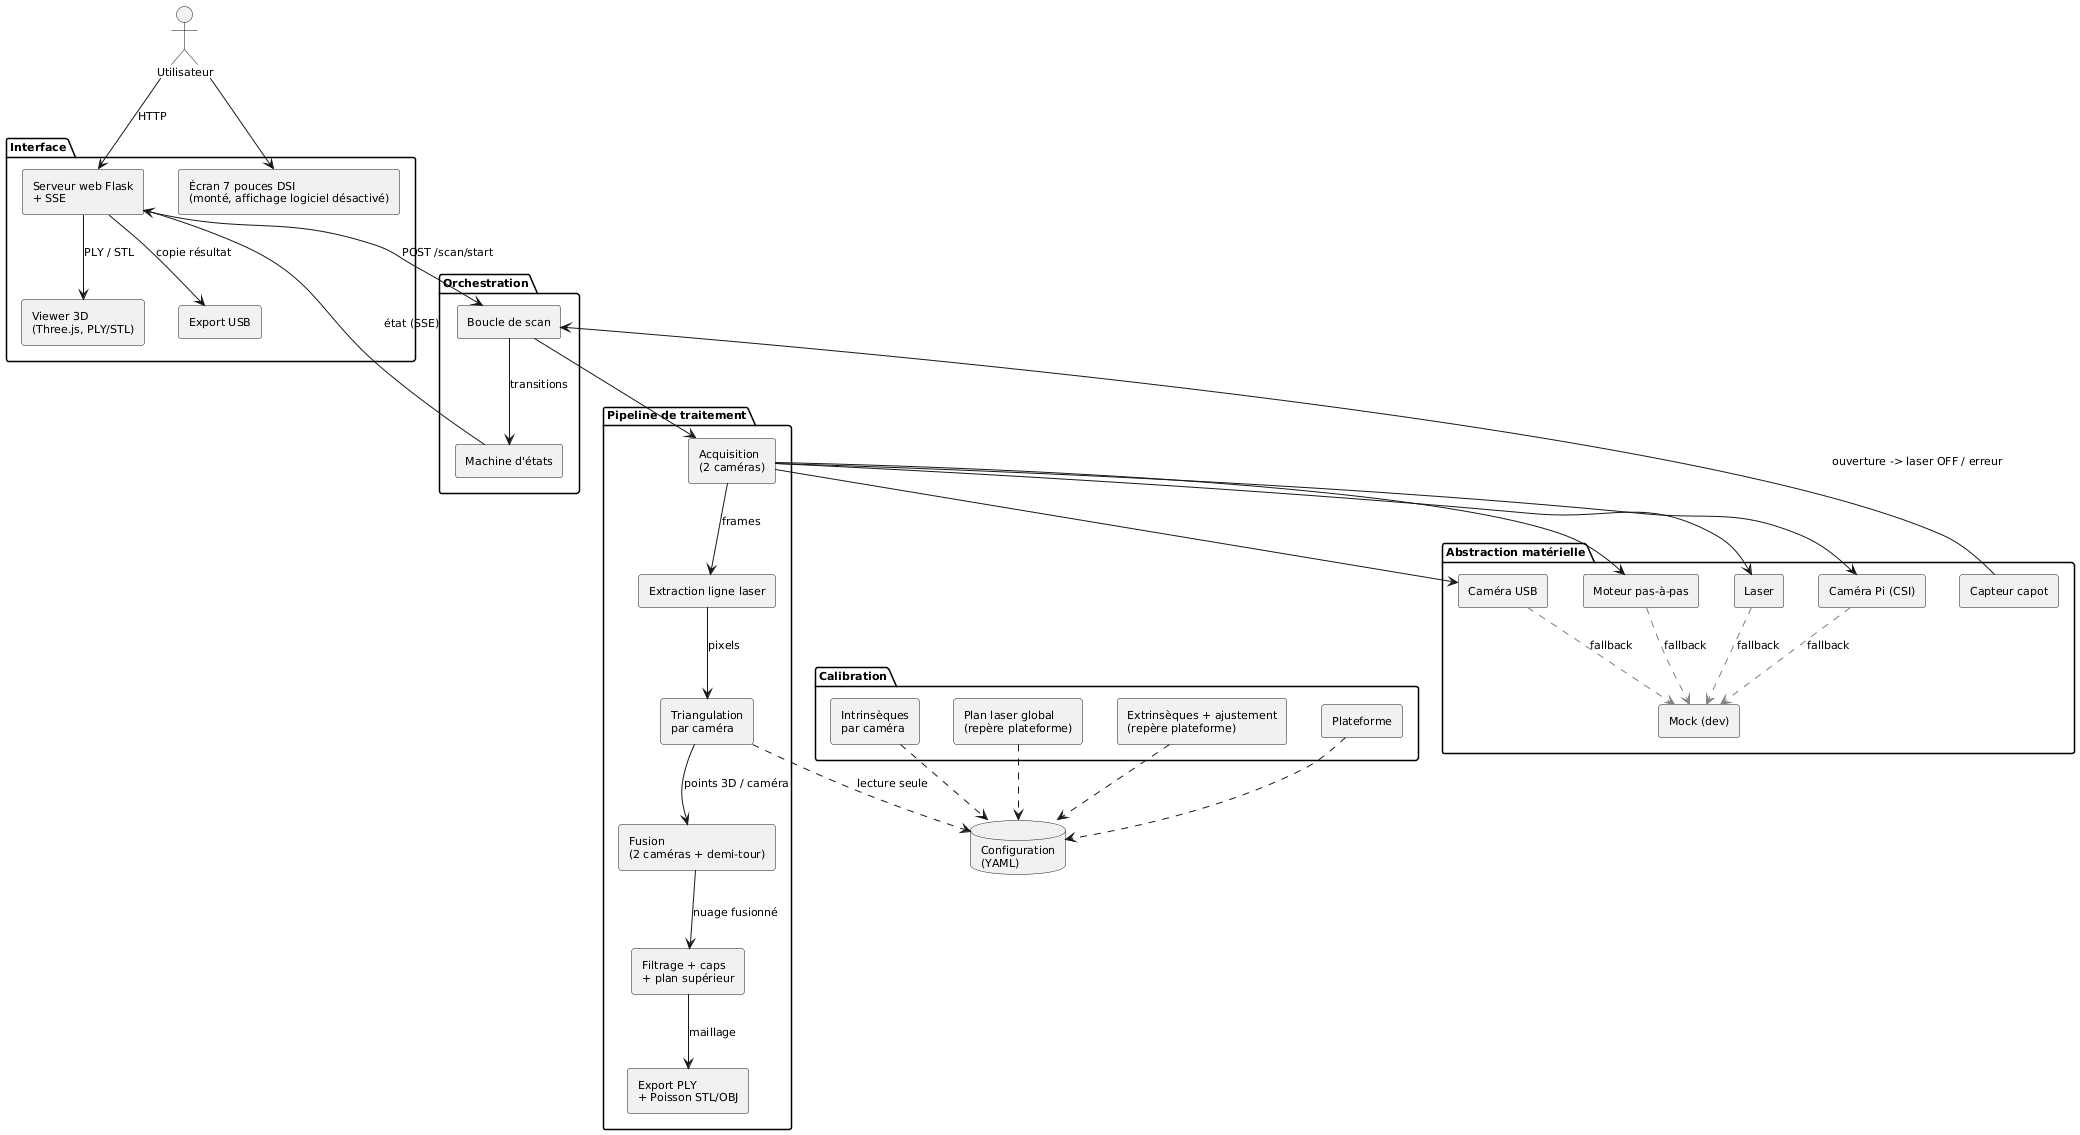
\includegraphics[width=\linewidth]{diagrams/architecture_composants.png}
  \caption{Architecture logicielle — vue des composants et flux de données.}
  \label{fig:archi-composants}
\end{figure}

\subsubsection{Modules}

\begin{table}[H]
  \centering
  \begin{tabular}{@{}p{3.5cm}p{10.5cm}@{}}
    \toprule
    \textbf{Module} & \textbf{Responsabilité} \\
    \midrule
    \texttt{hardware}       & Abstraction GPIO (moteur, laser, LEDs, caméra). Bascule automatique vers un \emph{mock} lorsque \texttt{gpiozero} est indisponible. \\
    \texttt{acquisition}    & Boucle capture : un pas moteur, allumage laser, capture image, extinction laser, sauvegarde. \\
    \texttt{processing}     & Extraction de la ligne laser (seuillage $G-R$, centroïde sous-pixel) et triangulation pixel $\rightarrow$ point 3D. \\
    \texttt{reconstruction} & Fusion des profils, filtrage d'\emph{outliers} par KDTree. \\
    \texttt{export}         & Génération STL / OBJ via \emph{convex hull} \texttt{trimesh}. \\
    \texttt{orchestration}  & Machine d'états et workflow de scan. \\
    \texttt{calibration}    & Calibration intrinsèque caméra (OpenCV) et plan laser. \\
    \texttt{interface}      & Serveur web Flask + SSE, affichage local TFT. \\
    \bottomrule
  \end{tabular}
  \caption{Modules logiciels et responsabilités.}
  \label{tab:modules}
\end{table}

\subsubsection{Flux de données}

La figure~\ref{fig:sequence-scan} détaille la séquence d'un cycle complet.
Pour un tour de plateau, 200 images sont acquises (pas de $1{,}8^\circ$),
chacune produisant un profil 2D, puis un nuage de points 3D par
triangulation avec le plan laser calibré.

\begin{figure}[H]
  \centering
  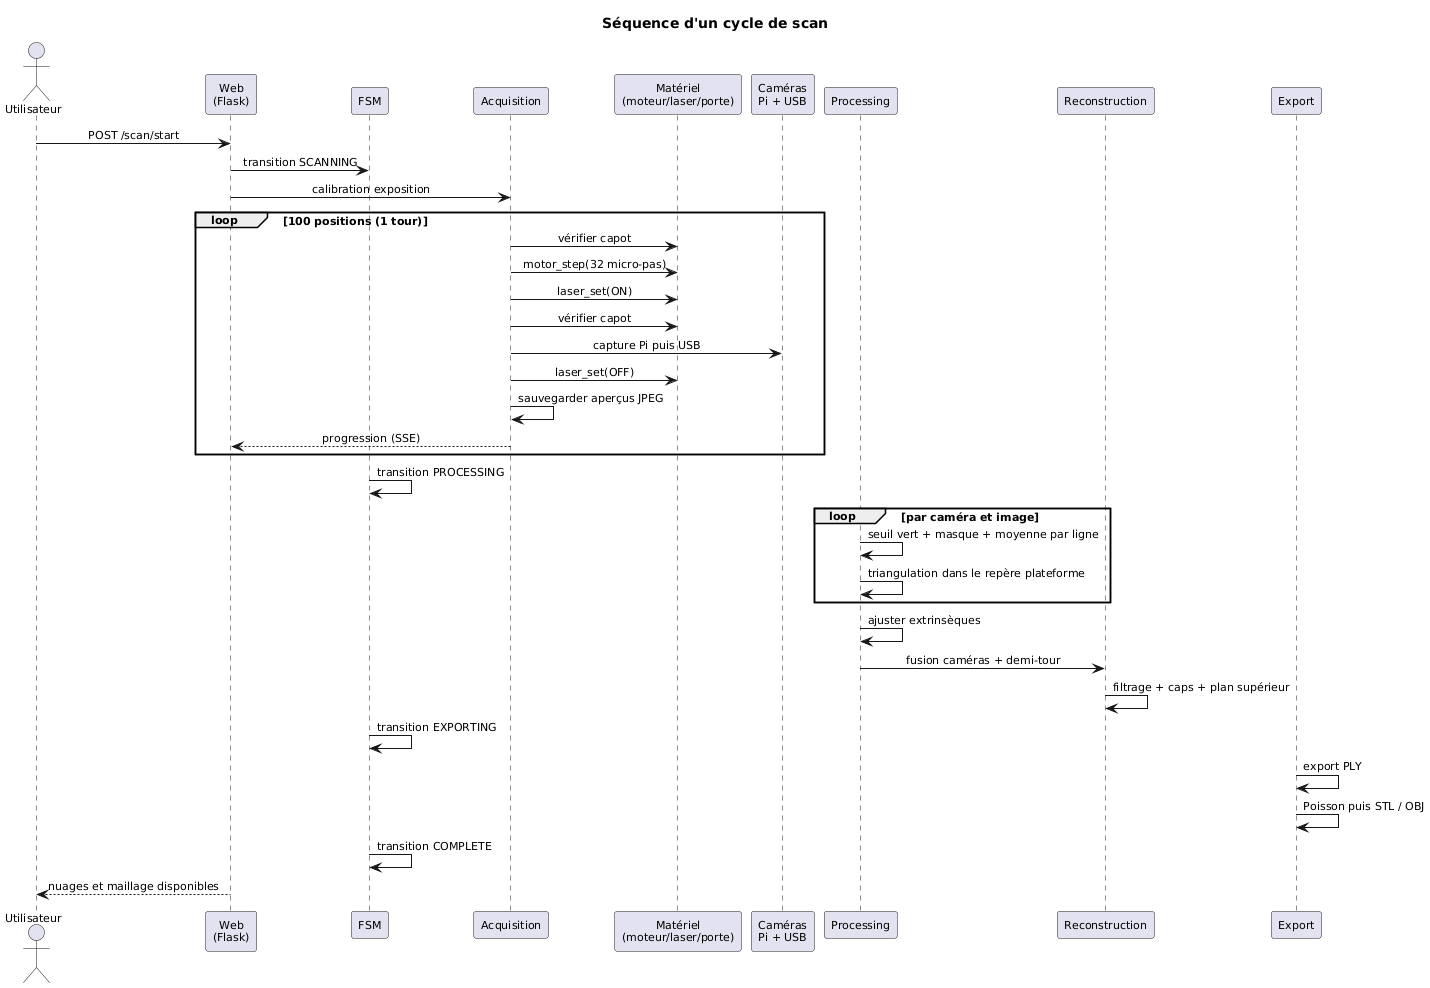
\includegraphics[width=0.95\linewidth]{diagrams/sequence_scan.png}
  \caption{Diagramme de séquence d'un cycle de scan.}
  \label{fig:sequence-scan}
\end{figure}

\subsection{Orchestration et machine d'états}

La FSM centralise les transitions légales et déclenche les effets de bord
associés (changement de LED, arrêt du laser en cas d'erreur). Les états
\texttt{IDLE}, \texttt{CALIBRATING}, \texttt{SCANNING}, \texttt{PROCESSING},
\texttt{EXPORTING}, \texttt{COMPLETE} et \texttt{ERROR} couvrent
l'ensemble du cycle de vie. Toute transition invalide lève une
exception plutôt qu'un état incohérent.

\begin{figure}[H]
  \centering
  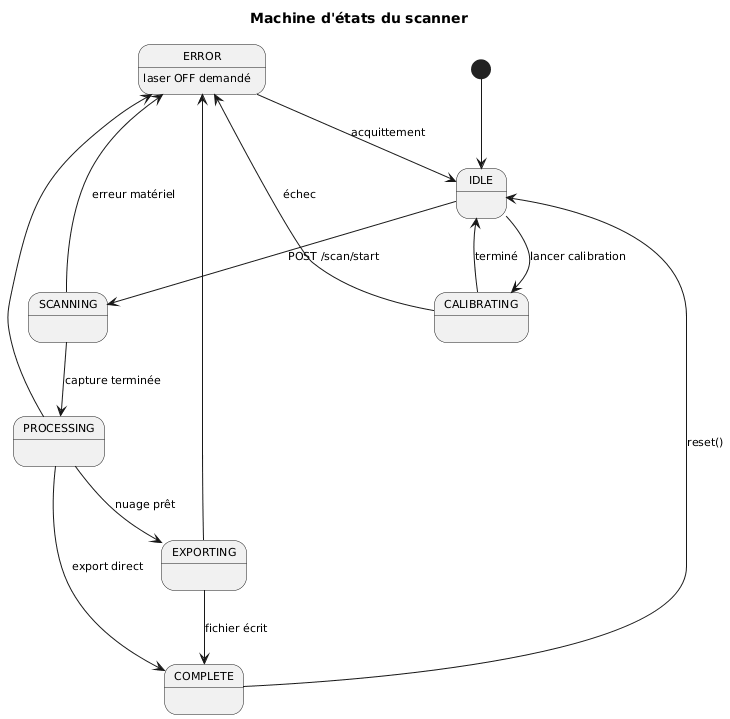
\includegraphics[width=0.85\linewidth]{diagrams/machine_etats.png}
  \caption{Machine d'états du scanner — transitions et signalisation LED.}
  \label{fig:fsm}
\end{figure}

\paragraph{Sécurité laser (exigence E19).}
Le laser est désactivé par défaut au démarrage. Un passage en
\texttt{ERROR} force sa coupure via un \emph{observer} de la FSM. Aucune
routine de calibration ne l'active sans confirmation. Un interrupteur de
porte (SW1, voir section électronique) complète la protection matérielle.

\subsection{Calibration}

Trois fichiers YAML, lus en lecture seule par le pipeline de scan,
stockent les paramètres calibrés :

\begin{itemize}
  \item \texttt{camera\_intrinsics.yaml} : matrice $3\times3$
        $(f_x, f_y, c_x, c_y)$ et coefficients de distorsion
        $(k_1, k_2, p_1, p_2, k_3)$, obtenus par damier + OpenCV.
  \item \texttt{laser\_plane.yaml} : équation du plan laser
        $[a, b, c, d]$ dans le repère caméra.
  \item \texttt{platform.yaml} : point de l'axe de rotation et nombre
        de pas par tour.
\end{itemize}

La règle d'immutabilité à l'exécution (le scan ne modifie jamais ces
fichiers) garantit la reproductibilité.

\subsection{Interface utilisateur}

L'interface web Flask (exigence \textbf{E10, E11}) expose les routes
nécessaires au lancement du scan, au suivi temps réel via Server-Sent
Events et au téléchargement du résultat. Un viewer Three.js charge
directement le STL binaire. Un afficheur TFT local reproduit l'état
courant pour un usage sans écran externe.

\subsection{Choix techniques}

\begin{table}[H]
  \centering
  \begin{tabular}{@{}p{4cm}p{4cm}p{6cm}@{}}
    \toprule
    \textbf{Besoin} & \textbf{Choix} & \textbf{Justification} \\
    \midrule
    Traitement d'image      & OpenCV          & Calibration caméra intégrée, léger sur Pi. \\
    Calcul numérique        & NumPy           & Standard scientifique Python. \\
    Filtrage de nuage       & SciPy KDTree    & Plus léger qu'Open3D sur Pi. \\
    Export maillé           & trimesh         & Support STL/OBJ sans dépendance GUI. \\
    GPIO                    & gpiozero        & API haut niveau, fallback \texttt{RPi.GPIO}. \\
    Interface web           & Flask + SSE     & Simple, SSE pour les mises à jour sans WebSocket. \\
    Viewer 3D               & Three.js        & Lecture native du STL binaire. \\
    Tests                   & pytest          & Standard, tous les GPIO mockés. \\
    \bottomrule
  \end{tabular}
  \caption{Bibliothèques et justifications.}
  \label{tab:choix-tech}
\end{table}

\subsection{Points ouverts}

\begin{itemize}
  \item Reconstruction concave (Poisson, \emph{alpha shape}) : actuellement
        \emph{convex hull}, suffisant pour un MVP mais limité pour les formes
        creuses. \emph{À compléter lors de la V2.}
  \item Export sur clé USB : stratégie de montage automatique à définir.
  \item Performances de bout en bout à mesurer pour respecter la cible
        de scan $<$ 10\,min (besoin B4 du CDC V2) et la précision
        \textbf{E24} ($\leq 2$\,mm d'erreur absolue, $\leq 1$\,mm de
        répétabilité). \emph{Mesures terrain à reporter.}
\end{itemize}

\section{Prototype et résultats}

\subsection{État livré}

Le prototype réunit la boîte, le plateau motorisé, le laser, les deux
caméras, le PCB de commande, le capteur de capot, l'écran tactile et
l'interface web. Le pipeline réel produit des nuages PLY intermédiaires et un
maillage STL.

\begin{figure}[H]
  \centering
  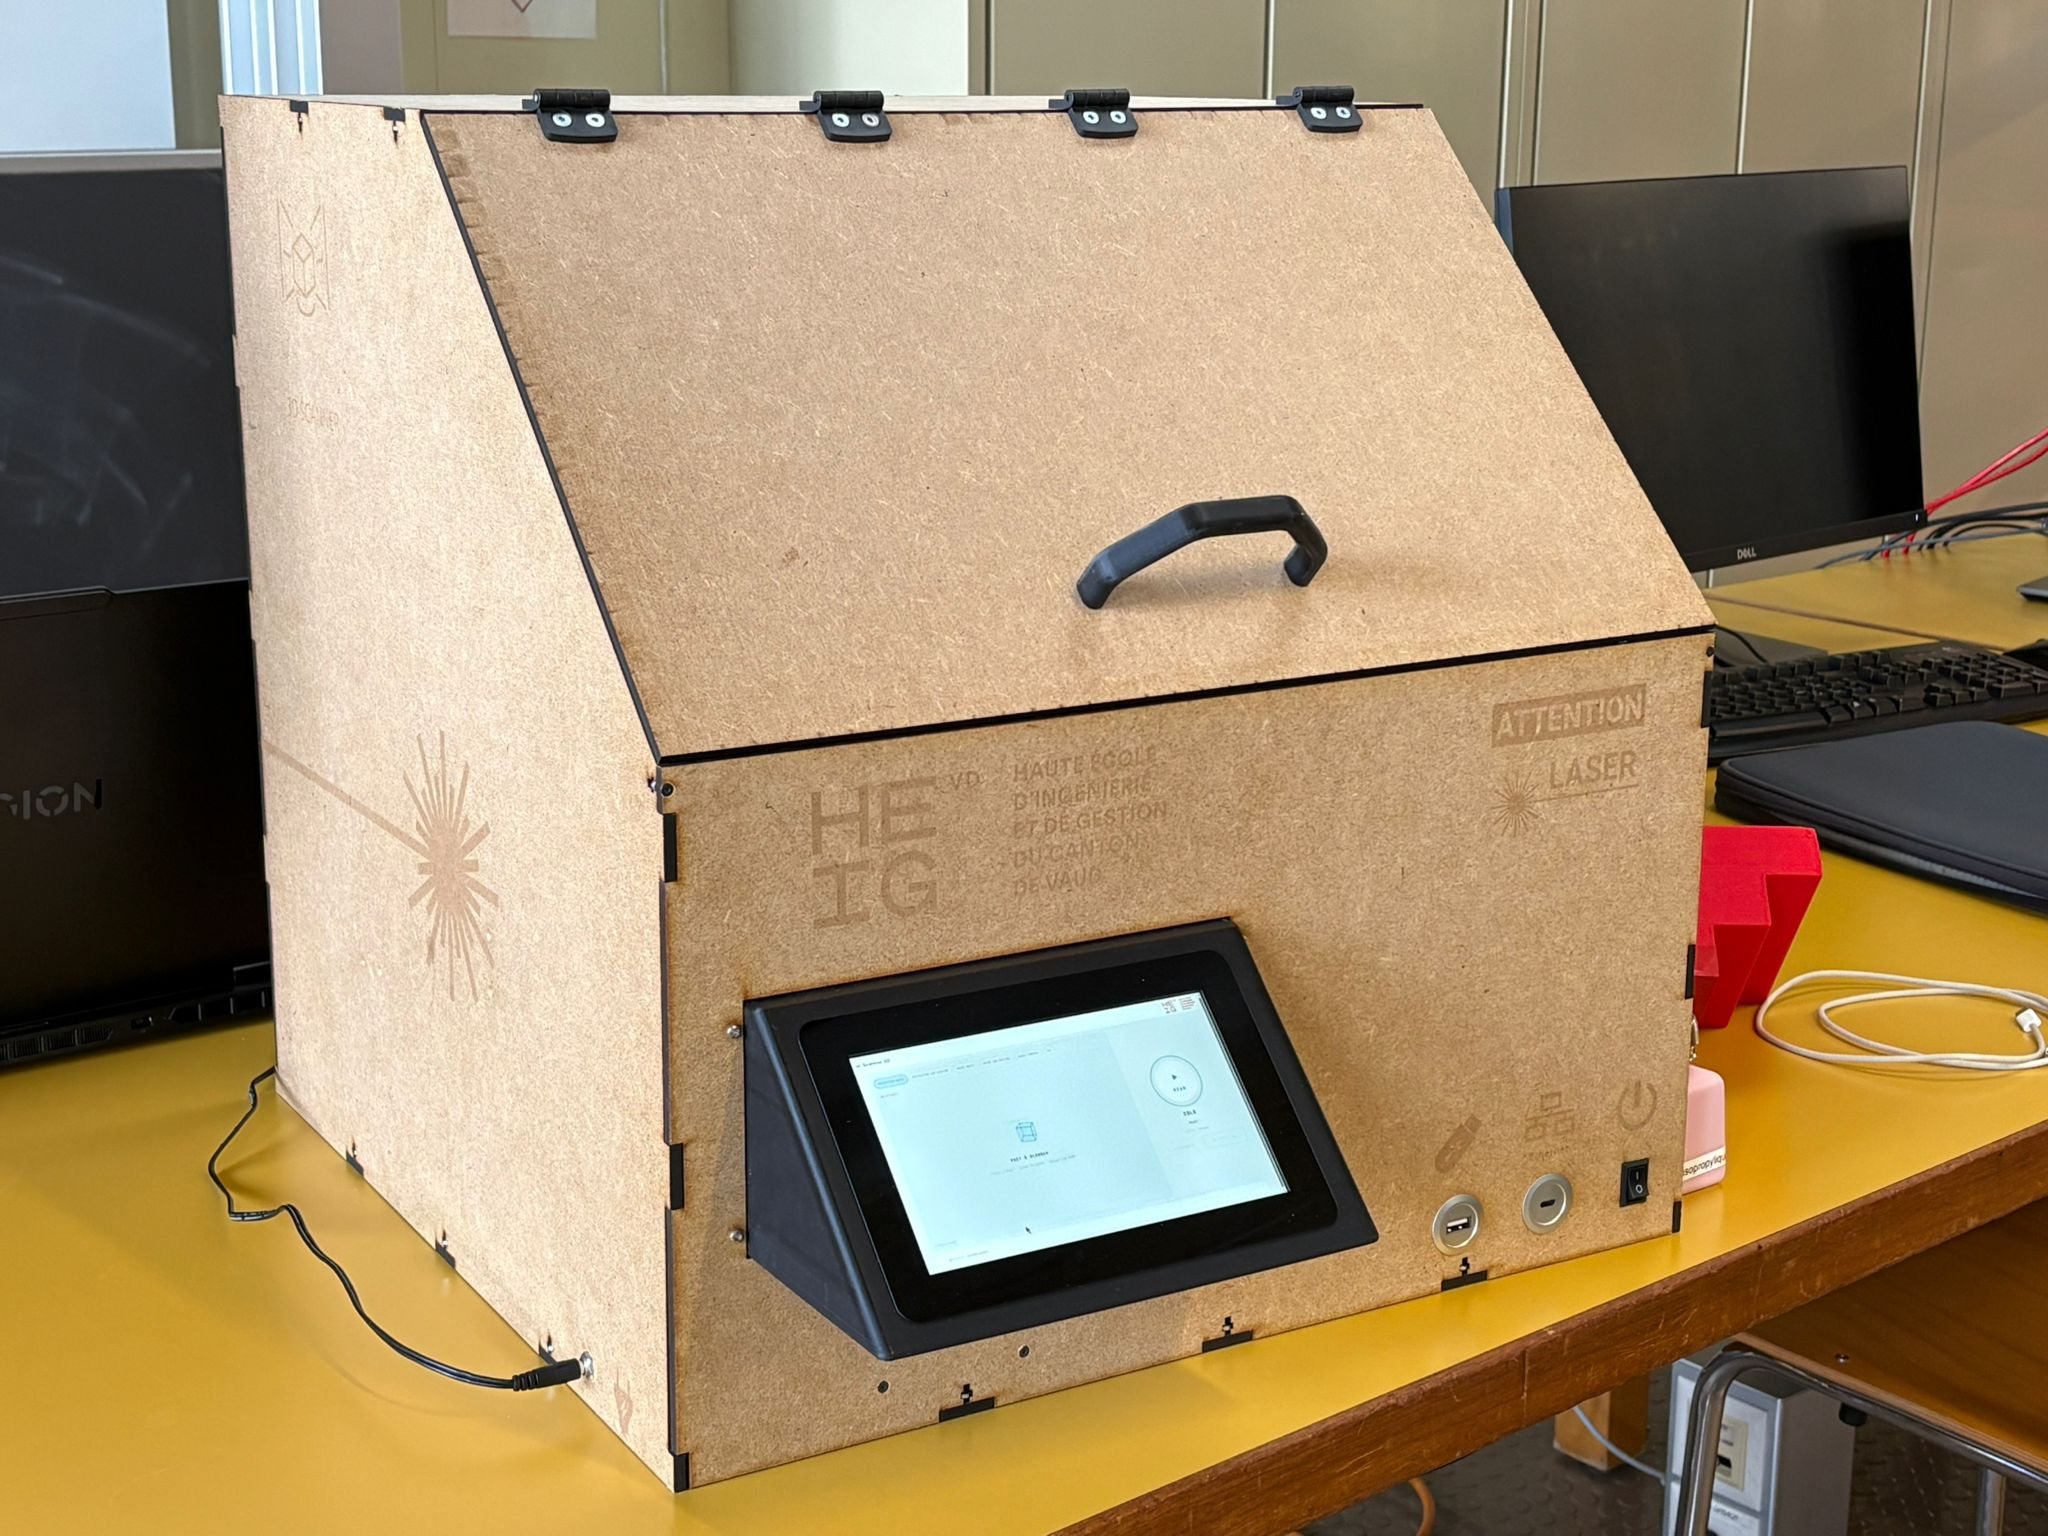
\includegraphics[width=0.6\linewidth]{images/boite_finale.jpeg}
  \caption{Vue extérieure du prototype final assemblé.}
  \label{fig:boite-finale}
\end{figure}

\begin{table}[H]
  \centering
  \small
  \begin{tabular}{@{}p{4.1cm}p{3cm}p{7cm}@{}}
    \toprule
    \textbf{Fonction} & \textbf{Statut} & \textbf{Justification} \\
    \midrule
    Acquisition à deux caméras & Démontrée & Pipeline matériel et captures par position. \\
    Interlock et arrêt laser & Testés & Capteur monté, contrôles avant activation et surveillance périodique à 100~ms. \\
    Extraction et triangulation & Démontrées & Nuages PLY produits par caméra. \\
    Fusion et maillage & Démontrés & Export Poisson STL disponible. \\
    Interface et export USB & Démontrés & Routes web, viewer et copie USB implémentés. \\
    \bottomrule
  \end{tabular}
  \caption{État des fonctions et validations.}
  \label{tab:maturite}
\end{table}

\subsection{Résultats}
\label{sec:prototype-resultats}

Un cycle complet, depuis le lancement jusqu'à l'export, a été chronométré à
environ 8 minutes. L'objectif O3 est donc atteint pour la configuration testée.
Les deux points de vue récupèrent davantage de zones sur les formes anguleuses
qu'une acquisition mono-caméra.

\begin{figure}[H]
  \centering
  \begin{minipage}{0.45\linewidth}
    \centering
    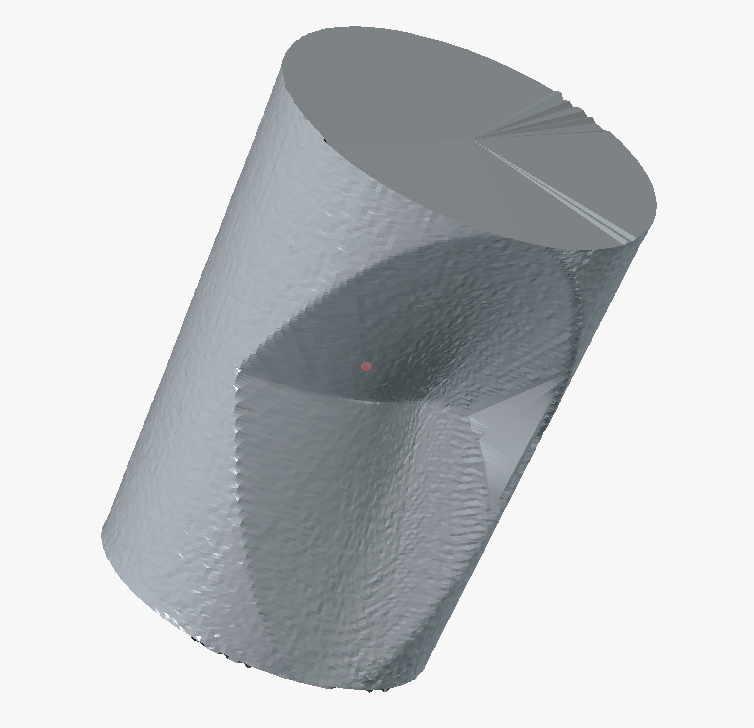
\includegraphics[width=0.85\linewidth]{images/screen_cylindre_stl.png}
    \\\small (a) Maillage d'un cylindre.
  \end{minipage}\hfill
  \begin{minipage}{0.45\linewidth}
    \centering
    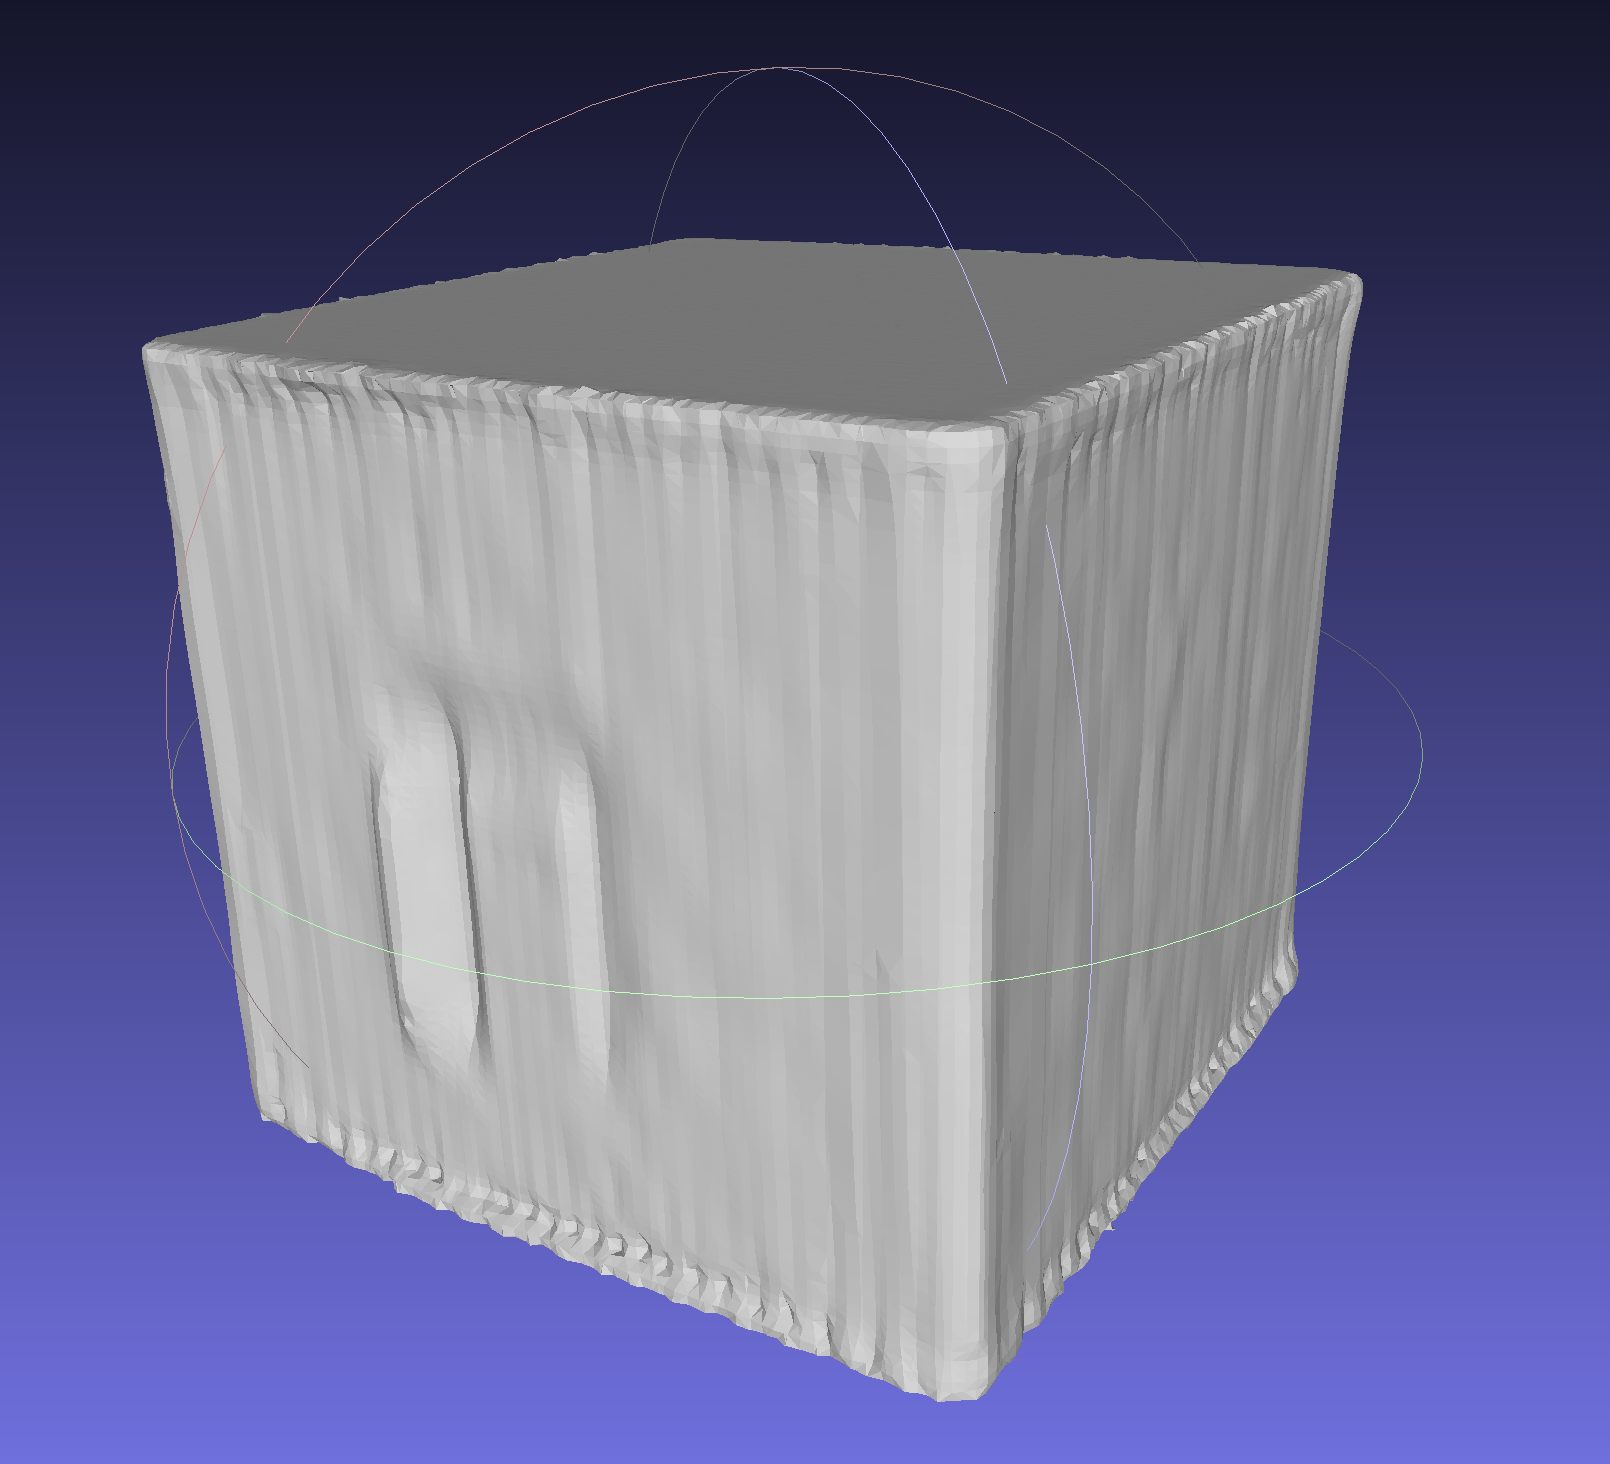
\includegraphics[width=0.85\linewidth]{images/cube_double_camera.png}
    \\\small (b) Résultat à deux caméras sur un cube.
  \end{minipage}
  \caption{Exemples de reconstructions produits par le pipeline final.}
  \label{fig:resultats-scans}
\end{figure}

\begin{figure}[H]
  \centering
  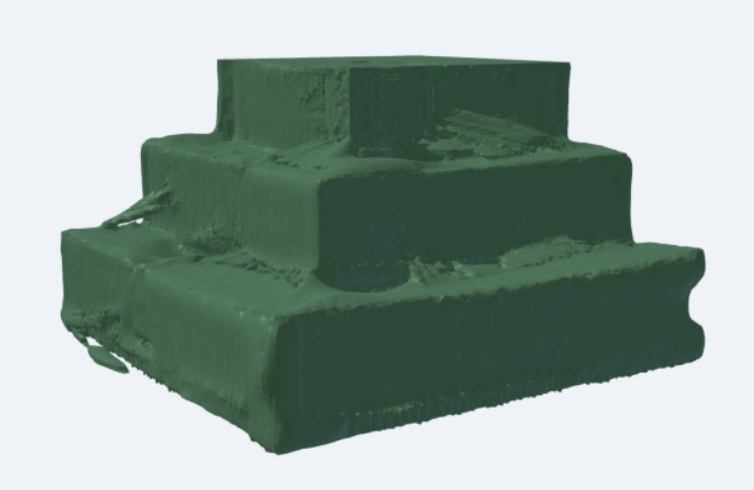
\includegraphics[width=0.68\linewidth]{images/resultat_escalier.png}
  \caption{Maillage obtenu pour la pièce en escalier. Les différents niveaux
  sont reconnaissables; des irrégularités restent visibles près des arêtes et
  dans certaines zones moins bien observées.}
  \label{fig:resultat-escalier}
\end{figure}

Les comparaisons dimensionnelles réalisées sur les pièces reconstruites
montrent une précision satisfaisante dans le plan horizontal: les dimensions
relevées suivant les axes $X$ et $Y$ restent généralement dans un intervalle
d'environ $\pm 2$\,mm par rapport aux dimensions de référence. L'échelle
verticale est en revanche moins fidèle et présente des écarts plus importants
sur l'axe $Z$. Cette différence semble liée à la plus forte sensibilité de la
hauteur reconstruite à l'ensemble de la chaîne géométrique, notamment au
réglage des poses, au plan laser et à la visibilité des surfaces horizontales.
Les essais disponibles ne permettent toutefois pas d'isoler une cause unique.
Le scanner restitue donc correctement la forme générale et les dimensions
dans le plan, tandis que la mesure suivant $Z$ demande encore une calibration
plus approfondie avant de pouvoir être considérée comme métrologique.

\begin{table}[H]
  \centering
  \begin{tabular}{@{}p{6cm}p{4cm}p{3.5cm}@{}}
    \toprule
    \textbf{Indicateur} & \textbf{Résultat} & \textbf{Cible} \\
    \midrule
    Cycle complet & $\approx$\,8\,min & $\leq 10$\,min \\
    Export STL & Produit & Obligatoire \\
    Coût réellement engagé & 133,83\,CHF & $\leq 300$\,CHF \\
    Dimensions extérieures & $500\times500\times500$\,mm & $\leq 500^3$\,mm \\
    \bottomrule
  \end{tabular}
  \caption{Résultats disponibles à la livraison.}
  \label{tab:perf-attendues}
\end{table}

\subsection{Limites}

La qualité dépend du réglage optique, des masques et de l'ajustement
extrinsèque. Les surfaces brillantes, très sombres, vertes ou cachées peuvent
dégrader l'extraction.

L'amélioration de la précision suivant l'axe $Z$ constitue un axe prioritaire
pour la suite du projet. Un travail complémentaire devra chercher à identifier
l'origine des écarts observés, en étudiant notamment la calibration du plan
laser, les poses extrinsèques des caméras et la propagation des erreurs dans la
triangulation. Une campagne de mesures sur plusieurs pièces étalons permettrait
ensuite de quantifier séparément la précision et la répétabilité sur les trois
axes.

Un mode de scan utilisant uniquement la caméra supérieure pourrait également
être avantageux pour les pièces simples et entièrement visibles depuis ce
point de vue. Il éviterait alors le regroupement de deux nuages et réduirait la
sensibilité du résultat aux extrinsèques relatives des caméras. L'acquisition
à deux caméras resterait toutefois essentielle pour les pièces plus complexes,
présentant des faces masquées ou des zones insuffisamment observées par une
seule caméra. Une évolution de l'interface pourrait ainsi permettre de choisir
le mode d'acquisition selon la géométrie de la pièce.

\section{Budget et coûts}

\subsection{Méthode}

Le budget du projet est présenté selon deux notions distinctes, conformément
à la grille d'estimation fournie au lancement du projet :

\begin{itemize}
  \item l'\textbf{estimation du coût du prototype} : ce que coûterait la
        réalisation si l'ensemble du travail était facturé aux tarifs
        horaires d'un bureau d'ingénierie (main d'\oe uvre, machines de
        fabrication et pièces achetées) ;
  \item le \textbf{coût réel pour l'école} : la dépense effectivement engagée.
        Les heures de travail des étudiants ne sont pas facturées, et les
        moyens de fabrication (impression 3D, découpe laser) ainsi qu'une
        partie des composants proviennent du stock du MakeLab. Le coût réel
        se résume donc aux pièces effectivement commandées, justifiées par
        les quittances.
\end{itemize}

Les tarifs horaires retenus sont ceux de la grille du cours : ingénieur HES
à 150\,CHF/h, mécanicien à 80\,CHF/h, impression 3D à 40\,CHF/h et découpe
laser à 50\,CHF/h.

\subsection{Estimation du coût du prototype}

Le temps de travail provient du planning final (\autoref{annexe:planning}) :
\textbf{361 heures} consommées au total. La répartition retenue distingue
les heures d'ingénierie (logiciel, électronique, électrique, gestion de
projet) des heures de mécanique (conception, fabrication et montage,
réalisées par le pôle ROCM). Les durées d'impression 3D et de découpe laser
correspondent au temps machine, estimé séparément.

\begin{table}[H]
  \centering
  \begin{tabular}{@{}p{5cm}r r r@{}}
    \toprule
    \textbf{Poste} & \textbf{Quantité} & \textbf{Tarif} & \textbf{Total} \\
    \midrule
    Ingénieur HES        & 314\,h & 150\,CHF/h & 47\,100\,CHF \\
    Mécanicien           & 47\,h  & 80\,CHF/h  & 3\,760\,CHF \\
    Impression 3D        & 15\,h  & 40\,CHF/h  & 600\,CHF \\
    Découpe laser        & 2\,h   & 50\,CHF/h  & 100\,CHF \\
    Pièces achetées      & ---    & ---        & $\approx$\,500\,CHF \\
    \midrule
    \textbf{Total estimé} & & & $\approx$\,\textbf{52\,060\,CHF} \\
    \bottomrule
  \end{tabular}
  \caption{Estimation du coût de développement du prototype, tarifs HES.}
  \label{tab:budget-estimation}
\end{table}

L'essentiel du coût estimé provient de la main d'\oe uvre d'ingénierie : le
projet est avant tout un travail de conception et de développement
logiciel. Le coût matériel reste marginal devant le coût en temps.

\subsection{Pièces achetées — nomenclature}

La nomenclature ci-dessous distingue les composants \emph{commandés} pour le
projet (justifiés par les quittances en annexe) des composants \emph{issus
du stock} du MakeLab, dont le prix est estimé au prix de marché pour
l'estimation du prototype.

\begin{table}[H]
  \centering
  \begin{tabular}{@{}p{6.5cm}p{2.2cm}r p{2.3cm}@{}}
    \toprule
    \textbf{Composant} & \textbf{Origine} & \textbf{Prix} & \textbf{Réf.} \\
    \midrule
    Laser ligne vert VLM-520-56 (520\,nm) & Commandé    & 77.08\,CHF & DigiKey \\
    2$\times$ caméra USB OV9726 (720p)\textsuperscript{*} & Commandé & 17.60\,CHF & Galaxus \\
    Adaptateur Gigabit Ethernet USB-C      & Commandé    & 8.90\,CHF  & Galaxus \\
    Adaptateur encastrable USB-C BU-BU     & Commandé    & 15.90\,CHF & Galaxus \\
    Adaptateur de panneau USB-A f-f        & Commandé    & 13.70\,CHF & Galaxus \\
    Contribution climatique                & Commandé    & 0.65\,CHF  & Galaxus \\
    \midrule
    Raspberry Pi 4 Model B                 & Stock       & $\approx$\,65\,CHF & --- \\
    Pi Camera Module 3                     & Stock       & $\approx$\,35\,CHF & --- \\
    Caméra USB Arducam IMX586              & Prêt        & $\approx$\,50\,CHF & --- \\
    Raspberry Pi Touch Display 2           & Stock       & $\approx$\,70\,CHF & --- \\
    Moteur pas à pas NEMA 17 (17HS3401)    & Stock       & $\approx$\,12\,CHF & --- \\
    Driver moteur DM320T                   & Stock       & $\approx$\,45\,CHF & --- \\
    Alimentation 24\,V 24\,W (Hama)        & Stock       & $\approx$\,25\,CHF & --- \\
    Convertisseur 24$\to$5\,V LM2596       & Stock       & $\approx$\,4\,CHF  & --- \\
    Interrupteur, connecteurs, capteur capot & Stock     & $\approx$\,15\,CHF & --- \\
    PCB dédié (fabrication)                & Stock       & $\approx$\,15\,CHF & --- \\
    Matière (PLA, panneau MDF, visserie)   & Stock       & $\approx$\,30\,CHF & --- \\
    \midrule
    \textbf{Total estimé (prix de marché)} & & \textbf{$\approx$\,500\,CHF} & \\
    \bottomrule
  \end{tabular}
  \caption{Nomenclature des pièces et estimation des prix. Les prix « Stock » sont estimés au prix de marché ; ils n'entrent pas dans le coût réel pour l'école.}
  \label{tab:budget-bom}
\end{table}

\textsuperscript{*}\,Les deux caméras USB OV9726 ont bien été commandées et
payées (elles figurent donc dans le coût réel), mais n'ont \emph{pas} pu être
utilisées : leur angle d'ouverture, non précisé à la commande, s'est avéré trop
étroit ($\approx 40^\circ$) pour couvrir la zone de scan. La seconde caméra du
montage final est une \textbf{Arducam IMX586} prêtée par l'école, qui n'a donc
engendré aucune dépense.

\subsection{Coût réel pour l'école}

Les heures de travail ne sont pas facturées et les moyens de fabrication du
MakeLab ne génèrent pas de dépense supplémentaire. Le coût réellement engagé
se limite aux deux commandes passées pour le projet, dont les quittances
figurent dans les annexes.

\begin{table}[H]
  \centering
  \begin{tabular}{@{}p{8cm}r@{}}
    \toprule
    \textbf{Commande} & \textbf{Montant (TTC)} \\
    \midrule
    DigiKey --- laser ligne VLM-520-56          & 77.08\,CHF \\
    Galaxus --- caméras USB et adaptateurs       & 56.75\,CHF \\
    \midrule
    \textbf{Coût réel total}                     & \textbf{133.83\,CHF} \\
    \bottomrule
  \end{tabular}
  \caption{Coût réel engagé pour le projet (quittances en annexe).}
  \label{tab:budget-reel}
\end{table}

Le coût réel de \textbf{133.83\,CHF} respecte largement l'objectif
budgétaire \textbf{O5} (\(\leq\) 300\,CHF). Même en valorisant l'ensemble
des composants au prix de marché ($\approx$\,500\,CHF,
\autoref{tab:budget-bom}), le coût matériel reste du même ordre de grandeur
que l'objectif, l'écart provenant essentiellement de l'écran tactile et du
Raspberry Pi.

\section{Conclusion}

\subsection{Bilan intermédiaire}

À mi-parcours du projet, l'équipe a figé l'architecture globale du
scanner (mécanique, électronique, logiciel), validé les choix
techniques principaux et produit une version fonctionnelle du
pipeline logiciel en simulation. Les objectifs SMART définis en
introduction restent atteignables dans le cadre du budget
(\textbf{E16}) et du délai de livraison du 7\,juin\,2026
(\textbf{E22}).

\subsection{Revue des objectifs}

\begin{table}[H]
  \centering
  \begin{tabular}{@{}p{1cm}p{9cm}p{4cm}@{}}
    \toprule
    \textbf{Réf.} & \textbf{Objectif} & \textbf{Statut} \\
    \midrule
    O1  & Numériser un objet $\leq 150^3$\,mm, automatisé          & En cours (intégration) \\
    O2  & Export STL ou OBJ                                         & Fait (logiciel) \\
    O3  & Cycle de scan $\leq 10$\,min                              & À mesurer \\
    O4  & Prise en main $\leq 10$\,min, autonomie $\geq 90$\,\%     & À valider (essais utilisateurs) \\
    O5  & Budget $\leq 300$\,CHF                                    & Piloté \\
    O6  & Sécurité utilisateur (laser, mobile, matériaux)           & Conçu, à valider sur prototype \\
    O7  & Retour visuel LED / écran                                 & Fait (logiciel) \\
    O8  & Interface USB ou web, scan en $\leq 5$ actions            & Fait (web Flask + SSE) \\
    O9  & Erreur $\leq 2$\,mm, répétabilité $\leq 1$\,mm            & À mesurer (risque principal) \\
    O10 & Encombrement $\leq 500^3$\,mm, masse $\leq 15$\,kg        & En cours (mécanique) \\
    O11 & Objets sans cavité fermée, contre-dépouille $\leq 45^\circ$ & Accepté (limite triangulation mono-vue) \\
    \bottomrule
  \end{tabular}
  \caption{Revue des objectifs au rapport intermédiaire.}
  \label{tab:revue-obj}
\end{table}

\subsection{Résultats principaux}

\begin{itemize}
  \item Architecture logicielle modulaire testée et validée en
        simulation ; pipeline \emph{Acquisition $\rightarrow$
        Traitement $\rightarrow$ Reconstruction $\rightarrow$ Export}
        opérationnel.
  \item Schéma électrique figé, sécurité laser intégrée par
        construction (coupure en état \texttt{ERROR}, interlock
        porte).
  \item Répartition claire des responsabilités dans l'équipe et
        planification cohérente avec la date de livraison.
\end{itemize}

\subsection{Risques identifiés}

\begin{itemize}
  \item \textbf{Précision E24 (O9)} : risque technique principal.
        Mitigation : calibration soignée, moyennage temporel,
        filtrage KDTree, caractérisation du banc de mesure.
  \item \textbf{Intégration mécanique tardive} : impact sur les
        mesures de précision et l'essai utilisateur.
        Mitigation : produire un prototype mécanique simplifié au
        plus tôt pour débloquer l'intégration.
  \item \textbf{Approvisionnement des composants} : à surveiller
        pour ne pas retarder la phase T30.
\end{itemize}

\subsection{Perspectives}

Phase T30 (semaines 9 à 14) :

\begin{enumerate}
  \item Assemblage mécanique et câblage du prototype.
  \item Calibration caméra et plan laser sur matériel réel.
  \item Premier scan bout-en-bout, confrontation aux objectifs
        O3 (temps) et O9 (précision).
  \item Essai d'ergonomie (O4) et ajustements d'interface.
  \item Mesures de consommation et validation thermique.
\end{enumerate}

Phase T40 (semaines 13 à 16) : préparation des livrables (rapport
final, vidéo de démonstration, présentation).

\subsection{Commentaire personnel}

\emph{À compléter en fin de projet (retour d'expérience de
l'équipe).}

\section{Bibliographie}
\nocite{*}
\begingroup
\setlength{\emergencystretch}{2em}
\printbibliography[heading=none]
\endgroup

\section{Annexes}

\subsection{Planning du projet}
\label{annexe:planning}

Le planning ci-dessous présente la répartition détaillée des tâches entre
les membres de l'équipe, leur ordonnancement sur les 16 semaines du projet
et le temps effectivement consommé (361\,heures au total).

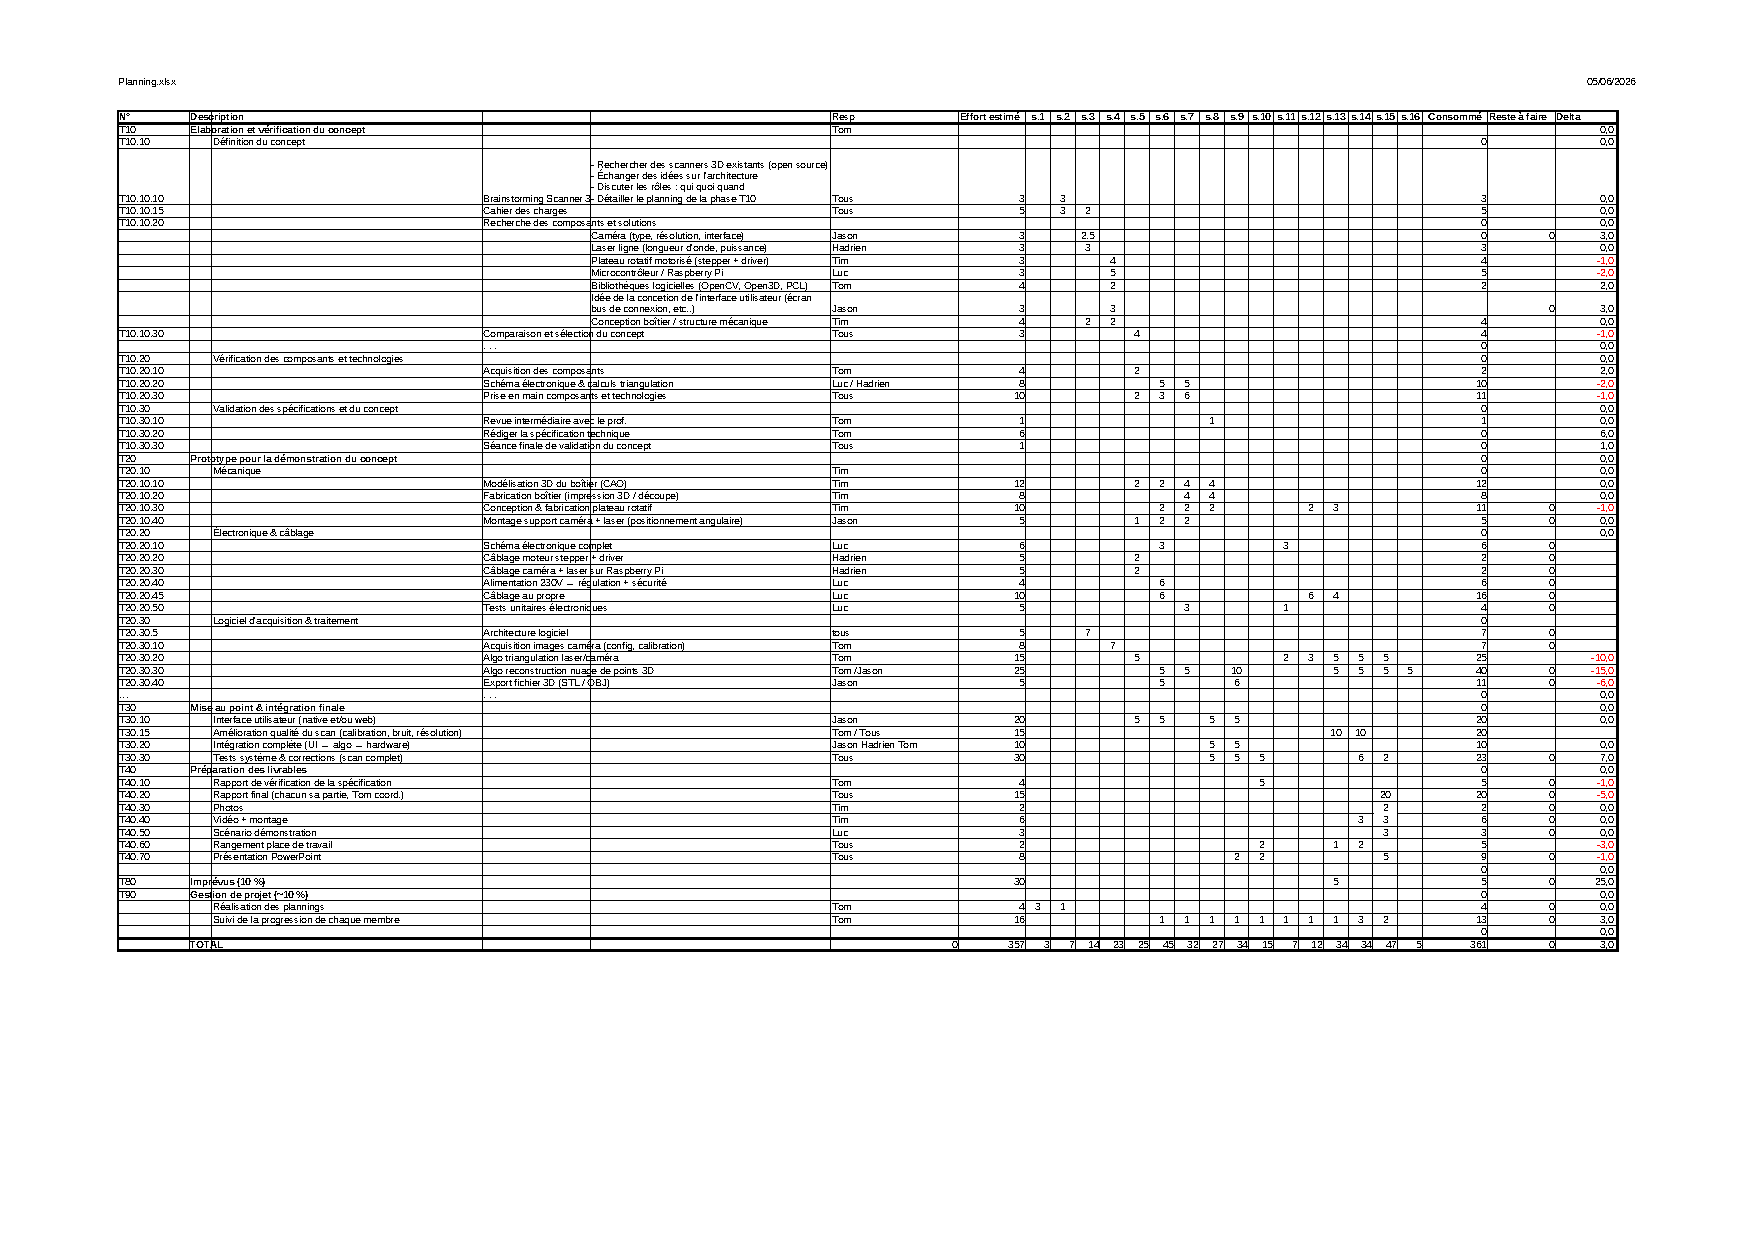
\includepdf[pages=-,pagecommand={},fitpaper=true]{assets/Planning.pdf}

\subsection{Quittances}
\label{annexe:quittances}

Les deux commandes passées pour le projet sont justifiées par les quittances
suivantes (cf. \autoref{tab:budget-reel}).

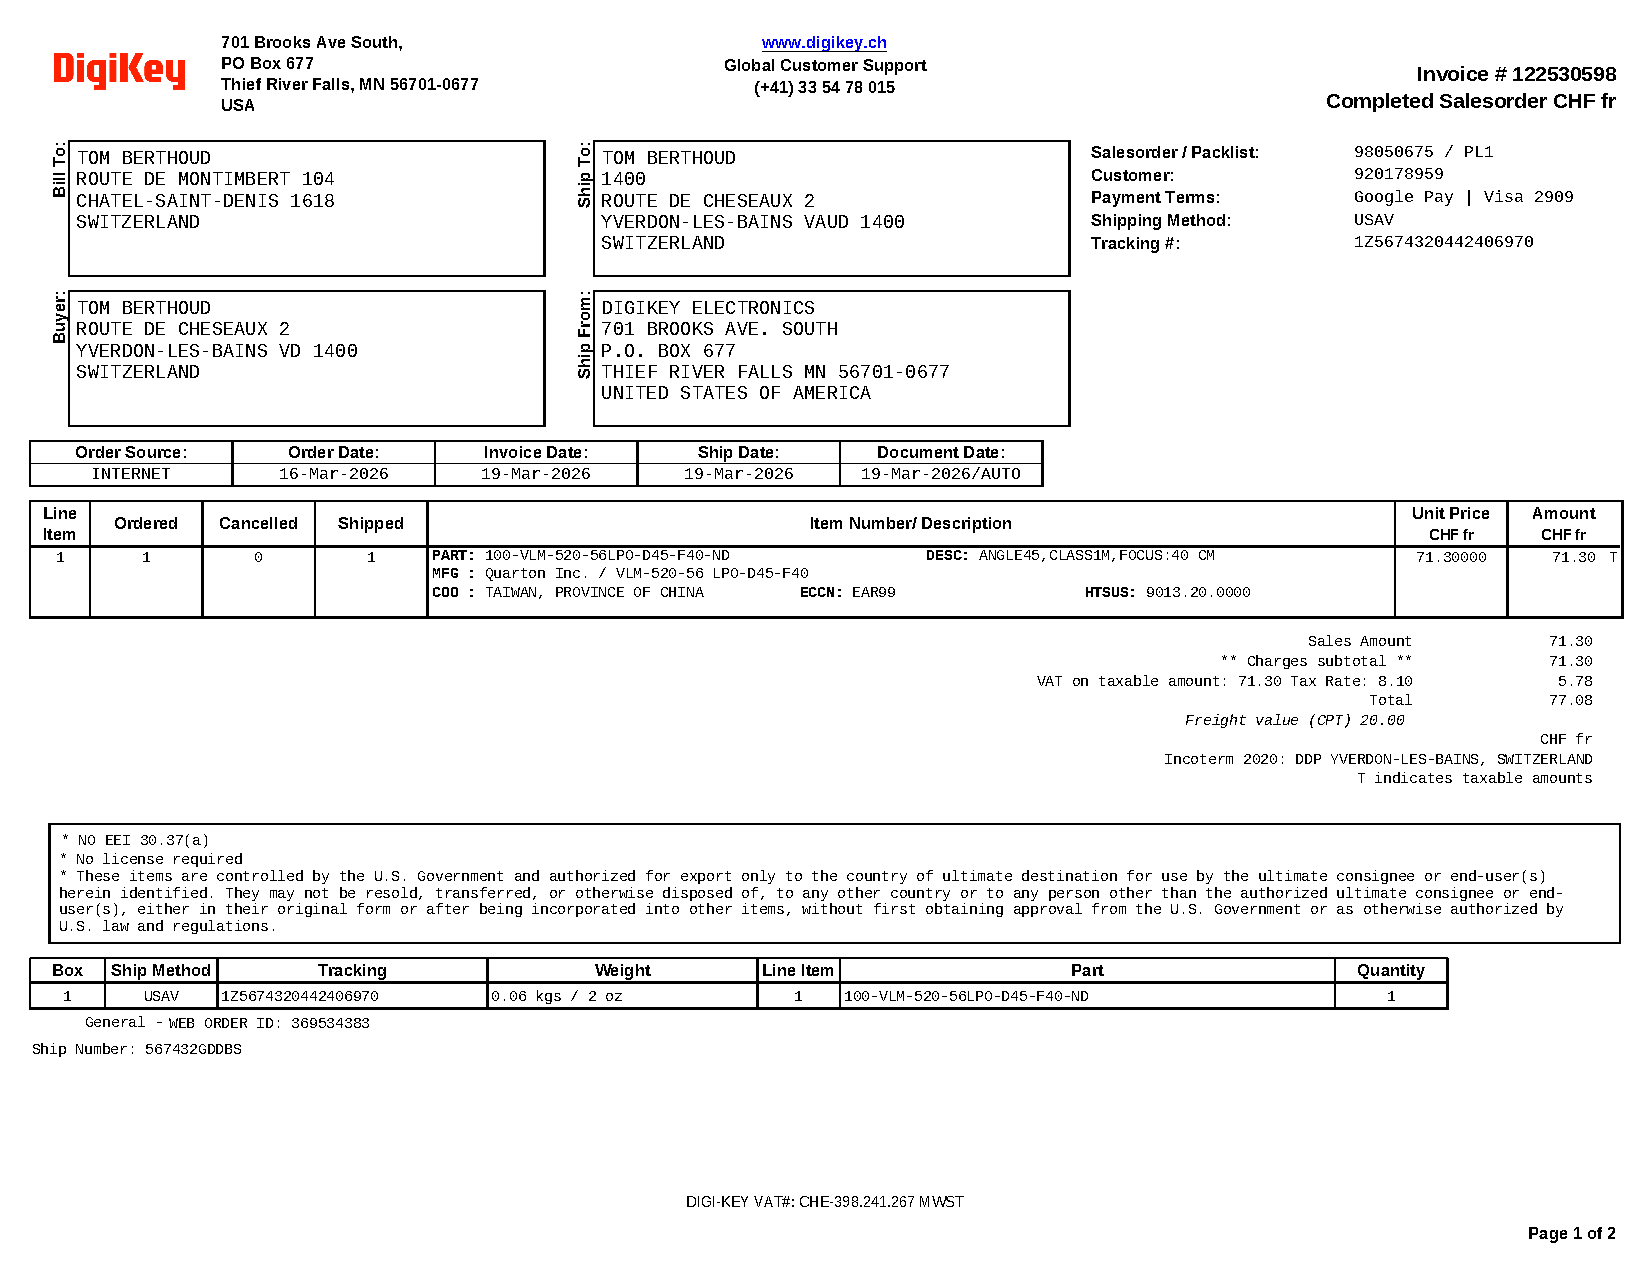
\includepdf[pages=-,pagecommand={},fitpaper=true]{assets/facturelaser.pdf}
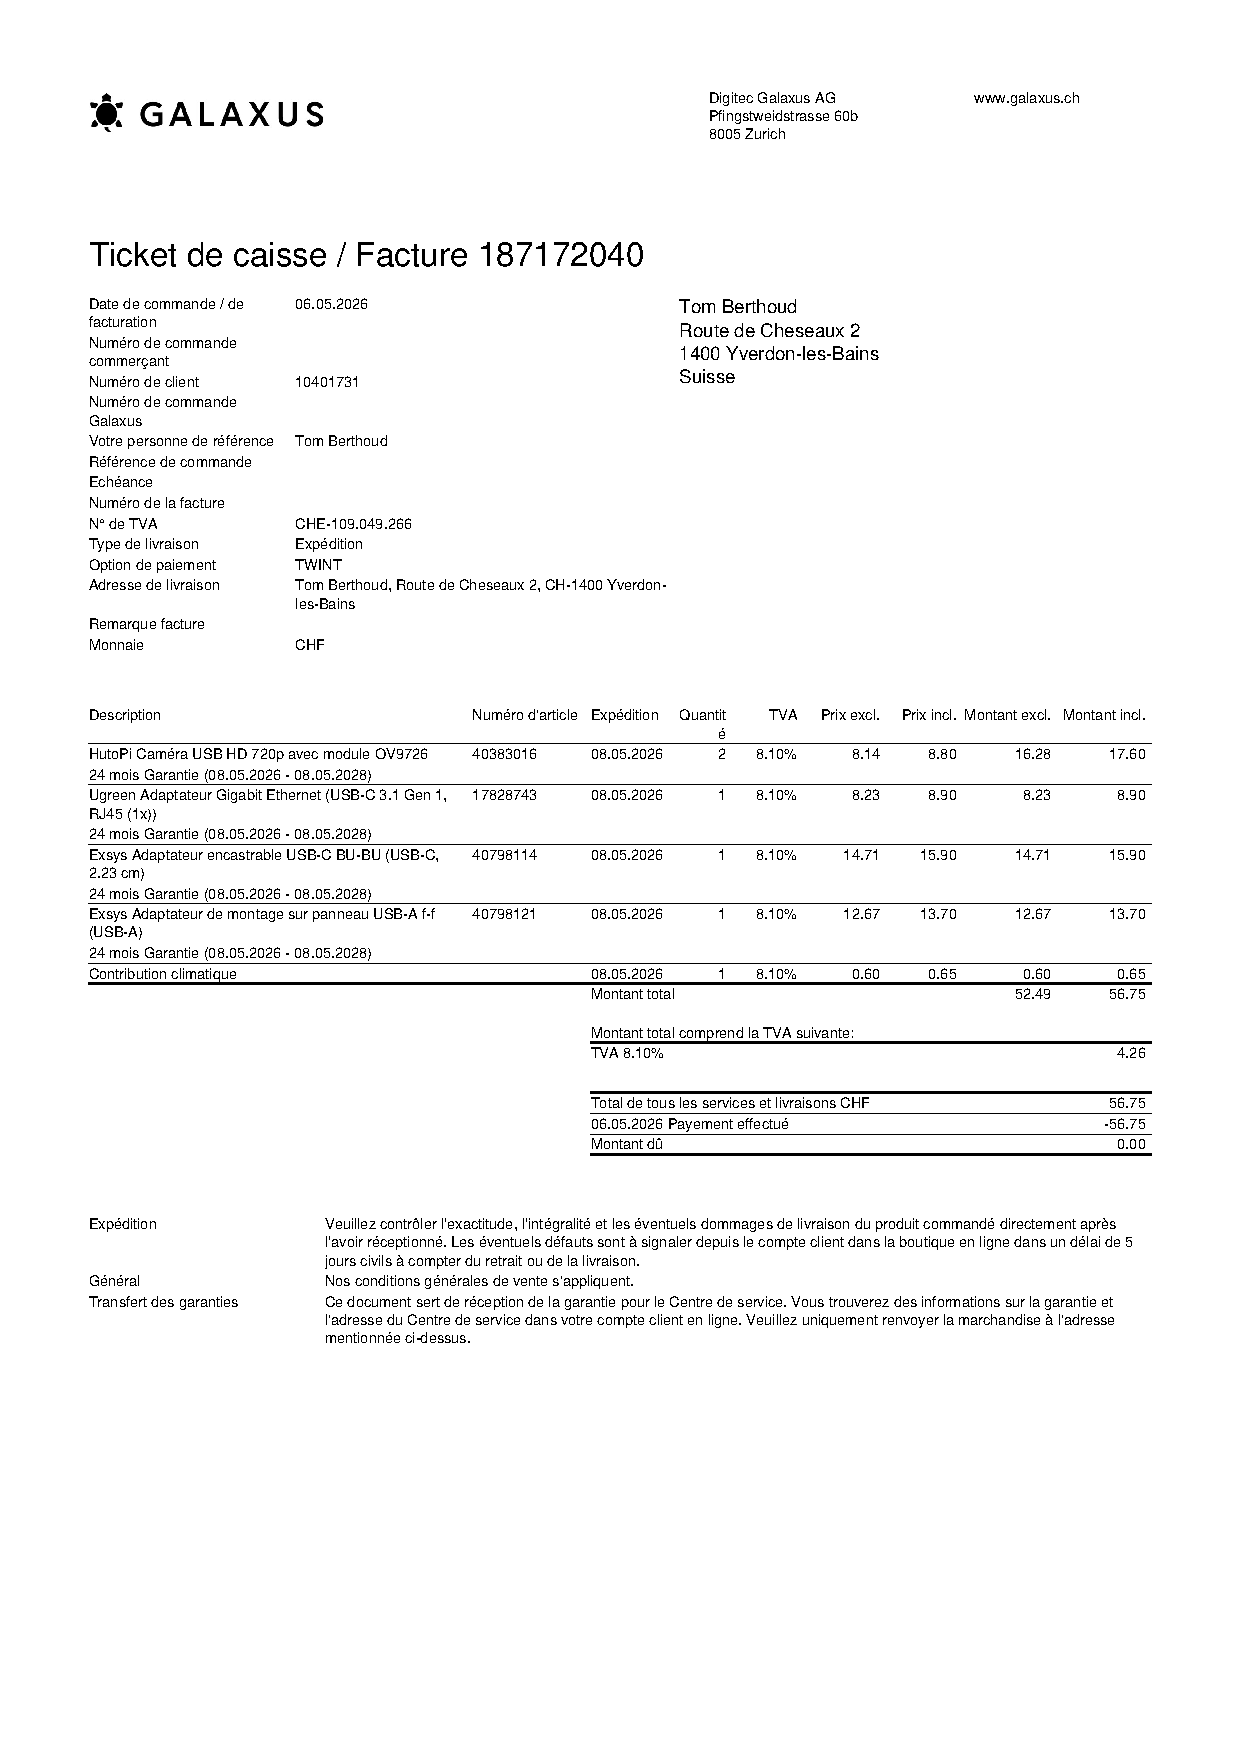
\includepdf[pages=-,pagecommand={},fitpaper=true]{assets/Galaxus_Ticket de caisse_187172040.pdf}


\end{document}
